\documentclass[12pt]{article}

\usepackage{amsmath}
\usepackage{amssymb}
\usepackage{graphicx}
\usepackage{hyperref}
\usepackage{geometry}
\geometry{a4paper, margin=1in}

\hypersetup{
    colorlinks=true,
    linkcolor=blue,
    filecolor=blue,      
    urlcolor=blue,
    citecolor=blue,
}

\title{Intro to AI \\ Assignment 2}
\author{Nikita Zagainov \\ DSAI-1}
\date{\today}

\begin{document}

\maketitle

\section{Implementation Details}
The algorithm for solving Sudoku is implemented in
\texttt{Python} and \texttt{C++} programming languages. 
The \texttt{Python} implementation is used for experiments 
and evaluation on test cases, while the \texttt{C++} 
implementation is used as submission on CodeForces.

For better availability of implementation details,
I provide the source code on github: 
\href{https}{Link}

\section{Evolutionary Algorithm Description}
\subsection{Algorithm Flow}
The EA algorithm follows a standard flow 
consisting of initialization, selection, crossover, 
mutation, and replacement. Each step will be 
described in detail below.

\subsection{Fitness Function}
The fitness function evaluates how close a 
given Sudoku solution is to being correct. 
It considers the number of conflicts in rows, 
columns, and subgrids.

\subsection{Variation Operators}
The variation operators include crossover and 
mutation. Crossover combines two parent solutions 
to produce offspring, while mutation introduces 
random changes to maintain diversity in the 
population.

\subsection{EA Parameters}
The EA parameters include population size, 
crossover rate, mutation rate, and the number 
of generations. These parameters are crucial 
for the algorithm's performance and will be 
tuned based on experimental results.

\section{Experimental Setup}
\subsection{Test Cases}
We evaluated the genetic algorithm on various 
Sudoku test cases with different numbers of 
givens and complexity levels. The test cases 
were divided into easy, medium, hard, and 
expert levels.

\subsection{Evaluation Criteria}
The evaluation criteria include the average and 
maximum population fitness at the final 
generations. We conducted at least 10 tests for 
each number of givens, ranging from 20 to 40. 
For complexity levels, we conducted at least 
50 tests for each level.

\section{Results and Discussion}
\subsection{Statistics}
We present the statistics demonstrating the 
average and maximum population fitness at the 
final generations for different numbers of 
givens or complexity levels. The results are 
shown in the following plots.

\subsection{Fitness Plot}
\begin{figure}[h]
    \centering
    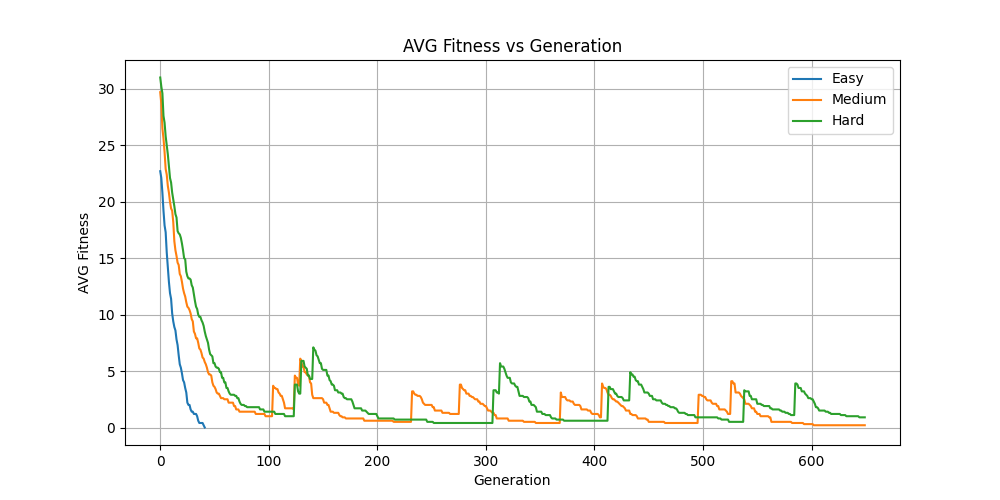
\includegraphics[width=\textwidth]{figures/plot.png}
    \caption{Average fitness value evaluated over 10 different Sudoku puzzles}
    \label{fig:avg_fitness}
\end{figure}


\section{Conclusion}
In conclusion, we have described the chosen 
EA algorithm and its components in detail. 
We provided statistical analysis and plots 
demonstrating the algorithm's performance on 
Sudoku puzzles with different numbers of 
givens and complexity levels. The results 
show that the algorithm performs better with 
more givens, as expected. Future work could 
involve further tuning of EA parameters and 
exploring other variation operators.

\section{References}
\begin{thebibliography}{9}
\bibitem{classification} 
Author. 
\textit{Title of the Classification Idea}. 
Journal/Conference, Year.
\end{thebibliography}

\end{document}